\documentclass[conference,a4paper]{IEEEtran}

\usepackage{fontspec}
\setmainfont{texgyretermes-regular.otf}[
  BoldFont=texgyretermes-bold.otf,
  ItalicFont=texgyretermes-italic.otf,
  BoldItalicFont=texgyretermes-bolditalic.otf
]
\usepackage{booktabs}
\usepackage{balance}
\usepackage{array}
\usepackage{tabularx}
\usepackage{microtype}
\usepackage{amsmath}
\usepackage{amssymb}
\usepackage{tikz}
\usetikzlibrary{arrows.meta,positioning,calc,automata,fit,backgrounds}
\usepackage{url}
\usepackage{xcolor}


\title{Timed-Automata Verification of Payload-Link Supervision, Watchdog Gating, and A/B Boot Policy in STM32 Flight Software}
% ---------------------------------------------------------------------------------------
% ICSEC 2026 requires DOUBLE-ANONYMOUS review submissions, so the review build carries
% placeholder author blocks with no real names or affiliations; the block count matches the
% camera-ready author count (six). Set \anonfalse for the camera-ready build.
% ---------------------------------------------------------------------------------------
\newif\ifanon
\anonfalse
% Camera-ready only: author contributions, funding and conflict-of-interest statements requested by the
% advisor on 2026-09-22. They add about eight lines and push the camera-ready build to seven pages, so they
% stay off until the conference's camera-ready page allowance is confirmed. Must remain false while \anontrue.
\newif\ifcontrib
\contribfalse

% IEEEtran V1.8b has no \linebreakand; this is the definition the IEEE conference template
% supplies for starting a second row of author blocks.
\makeatletter
\newcommand{\linebreakand}{%
  \end{@IEEEauthorhalign}
  \hfill\mbox{}\par
  \mbox{}\hfill\begin{@IEEEauthorhalign}
}
\makeatother

\ifanon
\author{\IEEEauthorblockN{Anonymous Author 1}
\IEEEauthorblockA{\textit{Anonymous Department} \\
\textit{Anonymous Faculty}\\
\textit{Anonymous University}\\
anonymous1@anonymous.edu}
\and
\IEEEauthorblockN{Anonymous Author 2}
\IEEEauthorblockA{\textit{Anonymous Department} \\
\textit{Anonymous Faculty}\\
\textit{Anonymous University}\\
anonymous2@anonymous.edu}
\and
\IEEEauthorblockN{Anonymous Author 3}
\IEEEauthorblockA{\textit{Anonymous Department} \\
\textit{Anonymous Faculty}\\
\textit{Anonymous University}\\
anonymous3@anonymous.edu}
\linebreakand
\IEEEauthorblockN{Anonymous Author 4}
\IEEEauthorblockA{\textit{Anonymous Department} \\
\textit{Anonymous Faculty}\\
\textit{Anonymous University}\\
anonymous4@anonymous.edu}
\and
\IEEEauthorblockN{Anonymous Author 5}
\IEEEauthorblockA{\textit{Anonymous Department} \\
\textit{Anonymous Faculty}\\
\textit{Anonymous University}\\
anonymous5@anonymous.edu}
\and
\IEEEauthorblockN{Anonymous Author 6}
\IEEEauthorblockA{\textit{Anonymous Department} \\
\textit{Anonymous Faculty}\\
\textit{Anonymous University}\\
anonymous6@anonymous.edu}}
\else
\author{\IEEEauthorblockN{Borworntat Dendumrongkul}
\IEEEauthorblockA{\textit{Department of Computer Engineering} \\
\textit{Chulalongkorn University}\\
Bangkok, Thailand \\
6632109921@student.chula.ac.th}
\and
\IEEEauthorblockN{Natdanai Hirunsirikul}
\IEEEauthorblockA{\textit{Department of Computer Engineering} \\
\textit{Chulalongkorn University}\\
Bangkok, Thailand \\
6732012721@student.chula.ac.th}
\and
\IEEEauthorblockN{Teejuta Sriwaranon}
\IEEEauthorblockA{\textit{Department of Computer Engineering} \\
\textit{Chulalongkorn University}\\
Bangkok, Thailand \\
6632102421@student.chula.ac.th}
\linebreakand
\IEEEauthorblockN{Pana Wanitchollakit}
\IEEEauthorblockA{\textit{Department of Computer Engineering} \\
\textit{Chulalongkorn University}\\
Bangkok, Thailand \\
6970210021@student.chula.ac.th}
\and
\IEEEauthorblockN{Phongsatorn Saisutjarit}
\IEEEauthorblockA{\textit{Department of Mechanical} \\
\textit{and Aerospace Engineering}\\
\textit{King Mongkut's University of}\\
\textit{Technology North Bangkok}\\
Bangkok, Thailand \\
phongsatorn.s@eng.kmutnb.ac.th}
\and
\IEEEauthorblockN{Pizzanu Kanongchaiyos}
\IEEEauthorblockA{\textit{Department of Computer Engineering} \\
\textit{Chulalongkorn University}\\
Bangkok, Thailand \\
pizzanu.k@chula.ac.th}
}
\fi


% The double-anonymous build carries a full placeholder author block, which costs about half a
% column on page 1; float, caption and table spacing are tightened to hold the six-page limit
% (arraystretch 0.92 since the 2026-09-22 acknowledgment addition, which otherwise spilled to page 7).
\setlength{\textfloatsep}{5pt plus 2pt minus 2pt}
\setlength{\floatsep}{5pt plus 2pt minus 2pt}
\setlength{\intextsep}{6pt plus 2pt minus 2pt}
\setlength{\dbltextfloatsep}{6pt plus 2pt minus 2pt}
\setlength{\abovecaptionskip}{2pt}
\setlength{\belowcaptionskip}{0pt}
\renewcommand{\arraystretch}{0.92}

\begin{document}
\maketitle

\begin{abstract}
Small-satellite flight software relies on interacting safety mechanisms -- poll/deadline supervision of a payload link, a task-health-gated hardware watchdog and a CRC-validated A/B bootloader -- whose worst-case behavior bench tests cannot bound; their composition in one prototype, checked against its own hardware traces, is not reported in the cited formal-verification papers. We model the three mechanisms of an STM32 flight-software prototype as UPPAAL timed automata, with constants copied from the C++ source, and verify safety, bounded-response and liveness properties in TCTL. Across twenty-one configurations and 368 formulas every verdict matches the oracle of expected verdicts: after confirmed fault onset the first timeout occurs within 603\,ms and OFFLINE within 1607\,ms, recovery completes within 516\,ms, a stalled critical task is detected within 952\,ms and forces a watchdog reset, and the boot policy never launches an unvalidated image. Model checking found a defect, fixed in source: a bypassed unconfirmed-boot limit. On the target, logic-analyzer timing keeps the poll period within 0.57\,ms of nominal, inside the assumed 2\,ms jitter, and traces a slip seen in host logs to the host's serial reader. Stall and boot-fault injection reproduce the boot defect and its fix and exposed a second defect the models assume away: bootloader and application kept retained state at different addresses, so a watchdog reset relaunched the application; after the fix every hardware outcome matches the model. The real C++ executed on the host stays within every bound, and replay of 90 frozen fault-injection trials refutes none. The guarantees concern the abstracted design, not the deployed C++, the RTOS or the HAL.
\end{abstract}

\begin{IEEEkeywords}
model checking, timed automata, UPPAAL, embedded flight software, watchdog, bootloader, payload link
\end{IEEEkeywords}

\section{Introduction}
Resource-constrained flight computers for CubeSat-class missions rely on a small set of deterministic safety mechanisms: a polling supervisor that detects a silent, corrupt, or late payload; a task-health registry that gates refresh of an independent hardware watchdog; and a bootloader that validates an image before jumping to it and otherwise falls back to a second slot or a safe beacon loop. A bench campaign shows only the paths it drove, and host timestamps cannot separate controller timing from serial and OS overhead: an earlier, unpublished hardware-in-the-loop (HIL) campaign on this prototype, whose frozen traces we reuse (Section~\ref{sec:conf}), observed the predefined markers in 30/30 trials per fault mode but could not claim controller-internal timing.

This paper asks what the design itself guarantees. We formalize the three mechanisms of an STM32 flight-software prototype (\ifanon name withheld for review; firmware not yet released\else WashiOS\fi) as UPPAAL timed automata~\cite{alur1994,larsen1997,behrmann2004} with constants copied from the source, verify properties with \texttt{verifyta}, execute the real C++ against the same properties, and use the frozen HIL traces not as the result but as offline consistency evidence for the models.

Contributions: (1)~timed-automata models of the three mechanisms with verified, attained worst-case detection, OFFLINE, recovery and stall-to-reset bounds, the delay-acceptance boundary, and safety and progress properties (Table~\ref{tab:props}); (2)~two defects, one found by model checking and one by on-target fault injection, and three design consequences, all confirmed in source (Section~\ref{sec:findings}); (3)~code-level evidence that the real C++ stays within the bounds (Section~\ref{sec:code}); (4)~on-target measurement of the assumed timing, with stall and boot-fault injection (Section~\ref{sec:hw}); (5)~offline replay of frozen, hash-verified traces under an anchor aligned with the model's clocks, which can refute agreement but does not establish conformance in the testing sense.
\textbf{Assurance limits.} We do not claim verification of the C++ implementation, correctness of the RTOS or vendor HAL, robustness to environmental or radiation effects, or any reliability estimate (Section~\ref{sec:discussion}).

\section{Related Work}
Timed automata~\cite{alur1994} and UPPAAL~\cite{larsen1997,behrmann2004} are the standard formalism and tool.
\textbf{RTOS semantics.} UPPAAL has been applied to conformance testing of an ARINC~653 RTOS~\cite{singh2021}, and model checking of the FreeRTOS Cortex-M4 port found errors reproduced on an STM32F429 board~\cite{lin2024}; both verify the kernel, whereas we verify application-level supervision above an abstracted kernel. UPPAAL has also been applied to satellite communication software~\cite{alencar2014}; link-supervision bounds are not reported in the cited paper.
\textbf{Scaling and properties.} State explosion is met with compositionality and abstraction~\cite{jensen2000}; our three networks stay small (at most 55\,462 states) because their coupling enters each as an input. Pattern catalogs generate observer automata for requirements beyond UPPAAL's fragment~\cite{vogel2023}.
\textbf{Model-to-code assurance.} Integrated formal verification~\cite{ge2018}, verified code generation from timed automata with runtime monitors~\cite{cho2025} and UPPAAL-TRON online testing~\cite{larsen2005} close the model--code gap more strongly than our replay of recorded traces, which shows only that a run did not contradict the model. Model checking has been combined with conformance testing and fault injection for space software~\cite{pontes2014}; fault injection~\cite{arlat1990,batista2019} is the empirical counterpart.
\textbf{The same mechanisms.} CAN arbitration and fault confinement~\cite{pan2014} and a heartbeat failure detector~\cite{johansson2020} have been verified in UPPAAL, neither with a poll/deadline supervisor and a consecutive-timeout threshold; an AUTOSAR Watchdog Manager has been verified by symbolic execution~\cite{ahmed2018}; a nanosatellite watchdog recovers restart-curable faults in flight~\cite{cutler2022}, and software-defined watchdogs act as eager deadlines~\cite{asch2025}. Those designs emphasize recovery, whereas the gate verified here is fail-safe (F2). Boot code has been verified for memory safety~\cite{cook2020} and secure boot~\cite{vasudevan2024}; slot selection, unconfirmed-boot limits and fallback across resets are not reported in the cited papers.

\section{Methodology}
\label{sec:method}
\subsection{System under study}
\label{sec:system}
The controller is a NUCLEO-G431RB (STM32G431RB, 128\,KiB flash, 32\,KiB RAM) running a FreeRTOS application with static allocation and no heap. Every constant below is quoted from the source and traced to its line in the artifact; Table~\ref{tab:trace} shows representative rows, including the source anchor of finding F4.

\textbf{Payload-link supervisor.} A 32-byte CRC-32 framed poll is sent every $P=500$\,ms. A valid response must arrive within $D=100$\,ms of the send instant; the deadline and the next poll are both anchored at that instant. On a timeout the consecutive-timeout counter increments and the link enters OFFLINE when it reaches $N=3$. A valid response resets the counter, sets ONLINE, and counts a recovery if the link was OFFLINE. A CRC-corrupted frame increments a counter but leaves the outstanding poll pending; a valid frame that arrives when no poll is pending is a sequence reject. The task services the controller once per $L=1$\,ms loop, receiving frames before evaluating the deadline.

\textbf{Watchdog gate.} Two critical tasks check in periodically: the heartbeat every 500\,ms with a 1500\,ms deadline, and the payload-link task every 100\,ms with an 800\,ms deadline. A watchdog task wakes every 50\,ms and evaluates the registry once 100\,ms have elapsed since the previous evaluation, expiring an entry whose last check-in is older than its deadline, and the first expiry records a watchdog-timeout and a safe-fail event in retained memory. The independent watchdog (IWDG), a hardware timer clocked by the internal low-speed oscillator (LSI, $\approx$32\,kHz) that resets the MCU unless refreshed, has a nominal 2.0\,s period (prescaler 16, reload 3999) and is refreshed only while all critical entries are healthy. On this target the safe-fail callback does not reset the processor; the IWDG does.

\textbf{A/B boot policy.} Each of two flash slots has a state: Empty, Valid, Pending (a staged image the application has not yet confirmed), Confirmed or Bad. On reset the bootloader recovers a CRC-protected fault log and boot metadata, kept in SRAM that survives a warm reset but not power loss, applies a confirmed-boot flag if set, refuses to boot if the active slot is Pending with a boot count above 3 or the fault log holds a check-in failure or watchdog timeout, validates the active slot's state, vector table and CRC-32, falls back to the other slot, and otherwise records a safe-fail and enters an LED beacon loop.

\begin{table}[t]
\centering\footnotesize
\caption{Scope per mechanism: what the model abstracts and what implementation evidence exists.}
\label{tab:scope}
\setlength{\tabcolsep}{3.5pt}
\begin{tabularx}{\columnwidth}{@{}>{\raggedright\arraybackslash}p{1.32cm} >{\raggedright\arraybackslash}X >{\raggedright\arraybackslash}X@{}}
\toprule
Mechanism & Abstracted in the model & Implementation evidence \\
\midrule
Payload link (Q) & wake-up jitter $J{=}2$\,ms; round trip derived from source; status-report block $S\in\{0,60\}$\,ms per 5\,s; lossless channel & on-target timing of $J$, $S$ and round trip; 15 MCU-timed trials; replay of 90 trials, nominal windows, delay sweep; C++ simulation \\
Watchdog gate (W) & task loop and poll as $50{+}100{+}J$; IWDG period as the LSI bracket $[1882,2170]$\,ms & 67 stall injections on the target; native unit tests; C++ simulation \\
Boot policy (B) & untimed; flash and application as environment choices; retained state survives a warm reset & SWD fault injection on the target; exhaustive run of the C++ policy; native test for F4 \\
\bottomrule
\end{tabularx}
\end{table}

\begin{table}[t]
\centering\footnotesize
\caption{Representative model-to-source rows (full trace in the artifact); line numbers are for the analyzed revision, before the F4 fix (Section~\ref{sec:findings}).}
\label{tab:trace}
\setlength{\tabcolsep}{3.5pt}
\begin{tabularx}{\columnwidth}{@{}>{\raggedright\arraybackslash}X l@{}}
\toprule
Model element & Source \\
\midrule
$P$, $D$, $N$ = 500, 100, 3 & \texttt{PayloadLinkController.hpp:32-34} \\
Idle$\to$Await; next poll anchored at send & \texttt{preparePoll()} \texttt{:53-73} (\texttt{:69}) \\
Receive before deadline evaluation & \texttt{PayloadLinkTask.hpp:45-47} \\
Mode read at decode; 1\,ms loop & \texttt{main.cpp:299-346}, \texttt{:454} \\
Status report every 5\,s (slip $S$) & \texttt{PayloadLinkTask.hpp:19}, \texttt{:180} \\
Refresh only if all critical tasks healthy & \texttt{Watchdog.hpp:61-65} \\
Limit 3, checked on active slot (F4) & \texttt{BootPolicy.hpp:16}, \texttt{:126-131} \\
Fallback, no limit re-check (F4) & \texttt{BootPolicy.hpp:86-92} \\
Shared retained region (F5 fix) & \texttt{.retained} in both linker scripts \\
\bottomrule
\end{tabularx}
\end{table}


\subsection{Payload-link model}
\label{sec:models}
The network has four templates. \emph{Controller} has clocks for the last poll, the outstanding poll and a received response; its transitions mirror \texttt{preparePoll}, \texttt{acceptResponse} and \texttt{service}, and a received frame is consumed at the next loop pass, before the deadline is evaluated. \emph{Payload} reads its mode when it decodes the request and answers after the round trip below, preceded by a configured delay $d$ in DELAYED mode, or not at all in SILENT mode, or with a corrupted CRC in BAD\_CRC mode. \emph{Status} blocks the link task, which then neither polls, evaluates the deadline nor consumes a frame, for at most $S$ once per 5\,s, at any phase. \emph{Host} reproduces the frozen trial protocol (Section~\ref{sec:confmethod}); its transitions are the confirmation events at which the comparison anchors start.

Abstractions: RTOS wake-up and ISR latency are bounded by $J{=}2$\,ms per wake-up (Section~\ref{sec:hw}). The round trip is derived from source: the request is decoded 2--9\,ms after the poll stamp (32-byte poll at 115200\,baud, the responder's 1\,ms loop, at most one blocking debug line), the response arrives 2--4\,ms later, and \texttt{HAL\_Delay}$(d)$ lasts $d$ to $d{+}1$\,ms. $S$ entered the model because, in the frozen 605\,s observation, host stamps show the poll schedule slipping by 10 to 54.5\,ms (median 30.4\,ms, $n{=}241$) at every status report; on the target the write delays no poll by more than 0.40\,ms and the slip comes from the serial reader (Section~\ref{sec:confmethod}), so $S{=}60$ is kept as an over-approximation at any phase. The channel is lossless except for the injected corruption; $d<P$. Q1, Q7, Q8, W1, W2 and every boot property do not involve $J$ or $S$, and every bound is a closed form in them (Table~\ref{tab:props}), so a re-measured value moves a bound without invalidating the proof. No $J$ covers blocking or priority inversion, which the code excludes (Section~\ref{sec:discussion}).



\subsection{Watchdog-gate model}
Two \emph{Task} instances check in with their periods and may be stalled by an \emph{Env} injector; a \emph{Supervisor} evaluates every 100\,ms with the source's strict-greater expiry test and refreshes the \emph{Iwdg} only when both are healthy; the IWDG resets when its clock reaches a value in $[1882,2170]$\,ms, derived from the datasheet LSI range of 29.5--34\,kHz over the full supply and temperature range~\cite{st2021ds12589}. Scenario~0 never stalls; Scenario~1 stalls one task after warm-up.





\subsection{Boot-policy model}
An untimed network (Fig.~\ref{fig:boot}): \emph{Boot} runs the policy over the retained variables (active slot, slot states, boot count, confirmed flag, retained critical fault, metadata corruption); \emph{App} may stall, setting the retained fault and resetting, reset cleanly, or, in a design variant, set the confirmed flag; \emph{Flash} corrupts an image, stages a Pending image in slot~B, or cold-starts the board, scrubbing retained SRAM. The shipped variant has no confirm edge (F1).



\begin{figure}[t]
\centering
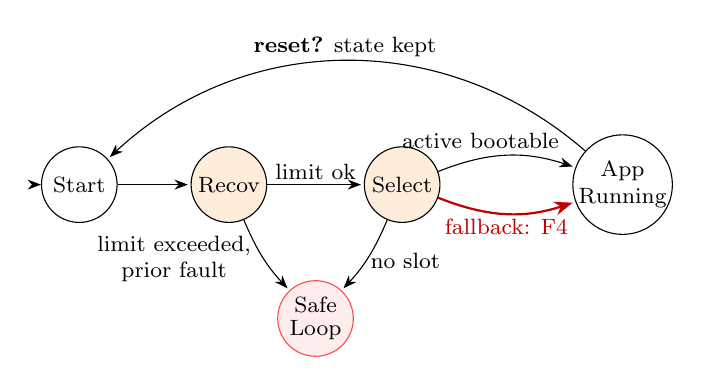
\begin{tikzpicture}[scale=1.0,transform shape,
  >=Stealth,shorten >=1pt,
  st/.style={draw,circle,inner sep=0pt,minimum size=9.6mm,font=\footnotesize,align=center},
  lb/.style={font=\footnotesize,inner sep=1.5pt,align=center},
  bad/.style={red!75!black,thick}]

% Every edge label sits beside its own edge, never across another one: the two launch edges
% bend apart around a common label corridor, and the two refusal edges form a V into SafeLoop
% with their labels on the outside of the V. The reset arc is bent to 42 and the launch label
% nudged left so the arc clears "active bootable" on its way down into AppRunning.
\node[st] (st0) at (0,0) {Start};
\node[st,fill=orange!14] (rc)  at (1.9,0) {Recov};
\node[st,fill=orange!14] (sel) at (4.1,0) {Select};
\node[st] (app) at (6.9,0) {\shortstack{App\\Running}};
\node[st,draw=red!70,fill=red!7] (safe) at (3.0,-1.7) {\shortstack{Safe\\Loop}};
\draw[<-] (st0) -- ++(-0.55,0);

\draw[->] (st0) -- (rc);
\draw[->] (rc) -- node[lb,above]{limit ok} (sel);
\draw[->] (sel) to[bend left=20] node[lb,above,pos=0.45,yshift=1pt,xshift=-7pt]{active bootable} (app);
\draw[->,bad] (sel) to[bend right=20] node[lb,below,pos=0.5,text=red!75!black]{fallback: F4} (app);
\draw[->] (rc)  to[bend right=10] node[lb,left,pos=0.52,xshift=-3pt]{limit exceeded,\\prior fault} (safe);
\draw[->] (sel) to[bend left=10]  node[lb,right,pos=0.55]{no slot} (safe);
\draw[->] (app) to[bend right=42] node[lb,above,pos=0.5]{\textbf{reset?} state kept} (st0);
\end{tikzpicture}
\caption{The A/B boot policy; shaded locations are committed (left without delay). The unconfirmed-boot check runs once, on the \emph{active} slot, leaving Recov; the red fallback edge activates the other slot and launches it without re-checking, so the launch inherits the accumulated boot count (F4).}
\label{fig:boot}
\end{figure}

\subsection{Properties}
\label{sec:props}
Table~\ref{tab:props} lists the properties referenced here; the 19, 11 and 14 formulas of the three models are in the artifact. UPPAAL checks three TCTL forms: \texttt{A[]}\,$\varphi$ ($\varphi$ holds in every reachable state), \texttt{E<>}\,$\varphi$ (some reachable state satisfies $\varphi$) and $\varphi \leadsto \psi$ (leads-to: every $\varphi$-state is eventually followed by a $\psi$-state). A bounded-response property is an \texttt{A[]} formula over a clock started at the confirmation event; its \emph{tightness twin} replaces $>$ by $\ge$ and is expected to fail, which shows that the bound is attained.

\begin{table}[t]
\centering\footnotesize
\caption{Properties. Bounds in ms, inclusive, for $J{=}2$; with a status report ($S{=}60$) in parentheses. Closed forms: Q2 $P{+}2J{-}2{+}D{+}L{+}S$; Q3 $N(P{+}J){-}2{+}D{+}L{+}J{+}S$; Q4 $P{+}2J{+}11{+}L{+}S$; W3 deadline${+}100{+}50{+}J$.}
\label{tab:props}
\setlength{\tabcolsep}{4pt}
\begin{tabularx}{\columnwidth}{@{}l l >{\raggedright\arraybackslash}X@{}}
\toprule
Id & Kind & Statement \\
\midrule
Q1 & safety & nominal, lossless, link up $\Rightarrow$ never OFFLINE \\
Q2 & bounded & fault confirmed $>$603 (663) $\Rightarrow$ timeout counted \\
Q3 & bounded & fault confirmed $>$1607 (1667) $\Rightarrow$ OFFLINE \\
Q4 & bounded & NORMAL confirmed $>$516 (576) $\Rightarrow$ ONLINE \\
Q5 & liveness & Restored $\leadsto$ ONLINE \\
Q7/Q8 & order & BAD\_CRC: CRC reject before first timeout; none yet $\Rightarrow$ ONLINE \\
Q9 & boundary & DELAYED $d{\le}85$ $\Rightarrow$ no timeout; $d{\ge}98{+}J{+}S$ $\Rightarrow$ late frames rejected; else both reachable \\
Q0/Q11 & progress & no deadlock; Awaiting $\leadsto$ Idle and Idle $\leadsto$ Awaiting \\
W1(a,b) & safety & no stall $\Rightarrow$ never reset (a), never critical failure (b) \\
W2 & safety & no IWDG refresh after a critical failure is recorded \\
W3 & bounded & stall detected within 952 (link), 1652 (heartbeat) \\
W5/W6 & liveness & stall $\leadsto$ IWDG reset, within W3 ${+}$ 2170 \\
B1/B2 & safety & never launch an unvalidated image or a non-bootable slot state \\
B3 & bounded & Pending active slot launched at most 4 times \\
B4/B5 & safety/reach & no valid image $\Rightarrow$ safe loop; safe loop reachable \\
B6 & safety & retained critical fault $\Rightarrow$ no relaunch before cold start \\
B7(,r) & finding & shipped app: Pending never Confirmed; reachable in the design variant (r) \\
B8(b,c) & finding & limit never bypassed (fails); only via fallback (b); next boot refused (c) \\
B9 & progress & Start $\leadsto$ AppRunning $\lor$ SafeLoop \\
\bottomrule
\end{tabularx}
\end{table}

\subsection{Consistency-evidence method}
\label{sec:confmethod}
The frozen traces come from a confirmation-gated protocol: a host injects a fault mode over the payload board's debug UART, counts the trial only after the payload confirms the mode, observes the controller console for 4\,s, restores NORMAL, waits for confirmation and observes for 3\,s; both serial channels are logged byte-exact with host timestamps and hash-inventoried. The campaign measured from the command send, which precedes the model's clock start; we measure from the \emph{confirmation anchor}, the host stamp of the payload's confirmation line, to the stamp of the controller's marker. Two uncertainties remain. The command-anchored intervals used a monotonic clock with a 15.6\,ms tick, which their disagreement with the wall-clock stamps (at most 15.4\,ms) reflects. The wall-clock stamps lag the lines they mark: the reader returns 64 bytes or a 50\,ms timeout, so a short line is stamped at the end of a read window, and a long one, such as a status report, ends a window early and shifts every later stamp. Against MCU-side edges with the same reader (Section~\ref{sec:hw}) the lag varies over 0 to 63.8\,ms, and an interval spanning a status report reads 496.5 to 553.0\,ms on the host but 498.1 to 501.2\,ms on the MCU: the slip above. The time bases agree: over 1319 periods the analyzer and host mean poll periods are 500.219 and 500.215\,ms. We declare a \emph{falsification floor} of 50\,ms: the replay refutes only violations larger than the floor and reports smaller excesses as unresolved, for MCU-timed runs to decide.


\section{Results}
\label{sec:results}
\subsection{Verified properties and bounds}
All configurations were verified with UPPAAL~5.0.0 (\texttt{verifyta}, rev.\ 714BA9DB) in one batch of 368 formulas, with outputs, instantiated models and SHA-256 inventory retained (Table~\ref{tab:verdicts}). Every verdict equals an oracle of expected verdicts stating which formulas must hold and which must fail; one prediction was corrected after the run. The largest state space is 55\,462 symbolic states (DELAYED 90 with a status report); no query took more than 2\,s of CPU on an Intel Core Ultra 7 155H.

\begin{table}[t]
\centering\footnotesize
\caption{Verification batch: 21 configurations, 368 formulas, all verdicts equal to the oracle (S satisfied, N not satisfied as expected; Q9c is two reachability formulas; ``+ status'' is $S{=}60$).}
\label{tab:verdicts}
\setlength{\tabcolsep}{3pt}
\begin{tabularx}{\columnwidth}{@{}l >{\raggedright\arraybackslash}X r >{\raggedright\arraybackslash}p{2.75cm}@{}}
\toprule
Model & Configuration & States & Verdicts \\
\midrule
payload & SILENT & 164 & 14 S, 5 N: Q2T, Q3T, Q4T, Q9c \\
payload & BAD\_CRC; DELAYED 100--250 & 210; 214 & as SILENT \\
payload & DELAYED 50 & 189 & 17 S, 2 N: Q9c \\
payload & DELAYED 90 & 1\,525 & 19 S (band) \\
payload & DELAYED 100, $J{\in}\{0,1\}$; $J{=}5$ & 242, 214; 1\,644 & as SILENT; 18 S, 1 N \\
payload & SILENT + status & 6\,109 & as SILENT \\
payload & BAD\_CRC, DELAYED 250 + st. & 8\,727; 9\,519 & as SILENT \\
payload & DELAYED 90 + status & 55\,462 & 19 S (band) \\
payload & DELAYED 110 + status & 10\,562 & 17 S, 2 N: Q4T, Q9c-2 \\
watchdog & no stall & 314 & 11 S \\
watchdog & one stall & 807 & 8 S, 3 N: W1a, W1b, W3T \\
boot & shipped app & 3\,035 & 12 S, 2 N: B7r, B8 \\
boot & design variant & 12\,547 & 11 S, 3 N: B7, B8, B8c \\
boot & F4 fix applied & 1\,988 & 13 S, 1 N: B7r \\
\bottomrule
\end{tabularx}
\end{table}

Every model satisfies \texttt{A[] not deadlock}; progress is stated explicitly (Q11, W5, B9) because the boot environment always offers an enabled edge. Each bound holds strictly and fails with $\ge$, so it is attained; it exceeds a naive derivation by one jitter term per poll period because the next poll is anchored at the actual send instant, which the model caught in our first estimate. In the DELAYED 90 band the recovery bound holds but is not attained (worst case 513\,ms), contrary to our oracle, which was corrected with the reason recorded. The first-timeout bound is $599+2J+S$\,ms; the acceptance edge $d\le 85$\,ms involves neither $J$ nor $S$, whereas the timeout edge $d\ge98+J+S$ moves with both, leaving a band of 86 to 99\,ms, or 86 to 159\,ms with a status report; at $J=5$\,ms, $d=100$\,ms becomes undetermined.

\subsection{Design findings}
\label{sec:findings}
Model checking produced one defect (F4) and made three design consequences precise (F1--F3); on-target fault injection found a second defect (F5). For F1 and F2 the models quantify behavior that source inspection had already identified; F4 was discovered by the checker.

\textbf{F1: the boot-confirmation path is unreachable in flight.} B7 holds in the shipped configuration and fails in the design variant: no application code writes the boot metadata, so a Pending slot can leave that state only through the attempt limit (B3, B8). The prototype is safe because slot~A is provisioned as Confirmed at build time.

\textbf{F2: critical stalls are fail-safe, not fail-operational.} W2 and W6 show that once a critical task expires the IWDG is never refreshed again and a reset follows within one IWDG period. B6 then shows the bootloader, seeing the retained watchdog-timeout event, enters the safe loop until a cold start -- a composed behavior the component tests did not show, and which the hardware exhibited only after F5 was fixed.

\textbf{F3: the effective delay boundary is below the nominal deadline.} Q9 proves acceptance for $d\le 85$\,ms and a timeout with sequence-rejected late frames for $d\ge100$\,ms (160\,ms with a status report); in between both outcomes are reachable. The frozen sweep accepted 90\,ms and rejected 100\,ms in every valid trial on three board pairs, and the executed controller code times out at 90\,ms in 13 of 7\,500 simulated trials, so the band is a property of the code, not of the abstraction.

\textbf{F4: the fallback path bypasses the unconfirmed-boot limit.} B8 fails in both boot configurations, and B8b localizes the violation to the fallback path. The limit check reads the \emph{active} slot; when that slot fails validation and the other is Pending, the fallback launch inherits the boot count accumulated by the confirmed slot. Every launch increments the count and only confirmation resets it, so a freshly staged Pending slot is launched at counts 0--3 and refused at 4 (B3), but after $k$ warm resets of the confirmed slot the fallback launches it at count $k$ unchecked and refuses it after $4-k$ launches -- after one once $k\ge3$ (B8c). The fix resets the attempt budget when the active slot changes; it was re-verified (B8 holds, other boot properties unchanged), a native regression test fails without it, and the exhaustive C++ run (Section~\ref{sec:code}) finds the violation on the pre-fix code only. On the target the pre-fix bootloader launches the fallback 3, 2 and 1 times for $k=1,2,3$ and the fixed one 4 times.

\textbf{F5: retained state was not shared.} B3, B6 and F4 assume that the fault log and boot metadata written before a warm reset are read after it. Each image kept its retained objects in its own uninitialized section: the bootloader at \texttt{0x20000018} (metadata) and \texttt{0x20000050} (fault log), the application its fault log at \texttt{0x20000088} and initialized data over both. After an IWDG reset the bootloader therefore found no fault and relaunched the application, and a Pending slot's boot count restarted whenever the application ran. The models and the host-level runs assume shared retained state; stall injection on the target exposed the gap. Both images now link one never-initialized region at fixed addresses (metadata, then fault log at +\texttt{0x40}) below all other RAM, and B3, B6 and F4 then hold on the target.

\subsection{Code-level conformance}
\label{sec:code}
We compiled the unmodified C++ of the three mechanisms on the host and ran it under the model's environment assumptions. The payload-link controller, frame codec and command parser run in a 1\,\textmu s discrete-event simulation of the two task loops, including every blocking UART write; over 287\,500 randomized trials the largest first-timeout, OFFLINE and recovery intervals are 596.7, 1598.6 and 506.4\,ms without a status report and 633.1, 1640.1 and 529.8\,ms with one, all within the bounds, and the delay edges match Q9. The real registry, watchdog and runner, stalled at every 1\,ms phase, detect a link stall within 870.8\,ms and a heartbeat stall within 1586.9\,ms (W3) and never refresh after a failure (W2). An exhaustive search of every retained state reachable under the boot model's environment (324 to 528 states) confirms B1--B4, B6 and B9 and finds B8 violated on the pre-fix code only. The task loops are restated by hand and the payload runs are sampled, so this is conformance evidence, not a refinement proof.

\subsection{On-target measurement and fault injection}
\label{sec:hw}
An instrumented build of the otherwise unchanged control code toggles a pin at every poll send, accepted frame, recovery, loop pass and console write, and the payload marks each confirmed mode change; an 8-channel logic analyzer at 1\,MSa/s gives target time to 1\,\textmu s. An F411 board replaced the unavailable G474 payload of the frozen campaign, which affects only the round trip and the MCU-timed trials. A stall build blocks one critical task 10\,s after boot. Boot faults are injected over SWD by corrupting a flash page and staging metadata in retained RAM; the bootloader's decision is read at the application's reset vector or after the application has run for 2\,s. Every MCU-timed interval in Table~\ref{tab:hw} lies within its bound, and $J{=}2$\,ms exceeds the measured period excess of 0.57\,ms more than threefold. Expiry to reset takes 1873.4 to 1874.6\,ms, less than the 1882\,ms IWDG minimum, because the IWDG period starts at the refresh of the previous evaluation, at least 100\,ms earlier; that instant was not probed.

\begin{table}[t]
\centering\footnotesize
\caption{On-target results (ms; $n$ in parentheses). Rows marked $^\dagger$ use the F411 payload; F5 rows before and after the shared retained region.}
\label{tab:hw}
\setlength{\tabcolsep}{3pt}
\begin{tabularx}{\columnwidth}{@{}>{\raggedright\arraybackslash}X l >{\raggedright\arraybackslash}p{4.05cm}@{}}
\toprule
Quantity & Model & Measured \\
\midrule
Poll period: all; with status & $P{+}J$ & 500.03--500.57 (1319); 500.08--500.40 (132) \\
Status write blocks link task & $S$ & 9.67--9.84 (132) \\
Poll to accepted frame$^\dagger$ & 4--16 & 6.01--8.02 (1320) \\
Fault to first timeout$^\dagger$ & ${\le}603$ & 113.6--593.5 (15) \\
NORMAL to recovery$^\dagger$ & ${\le}516$ & 159.0--503.5 (15) \\
Stall to expiry: link; heartbeat & W3 & 801.4--801.8 (24); 1091.9--1092.4 (23) \\
Stall to reset: link; heartbeat & W6 & 2675.3--2676.1; 2965.5--2966.4 \\
After IWDG reset & B6 & relaunch 47/47; fixed: safe loop 20/20, also after warm reset \\
Pending slot, resets & B3 & app run: 1 launch, then A; fixed, no app: 4, then refused \\
Fallback after $k{=}1,2,3$ resets & F4 & pre-fix 3, 2, 1; fixed 4, 4, 4 \\
\bottomrule
\end{tabularx}
\end{table}

\subsection{Consistency with frozen hardware traces}
\label{sec:conf}
The replay accepts every frozen dataset. In all 90 primary trials the predefined detector marker is the model's first observable event for that mode, and no trial recorded a controller restart marker. Both 65\,s nominal windows and the 605\,s observation show zero counter deltas (Q1). In the delay sweep the 3 rows at 50\,ms were accepted (Q9a), the 12 rows at 100 to 250\,ms timed out (Q9b), and the 3 accepted rows at 90\,ms fall in the undetermined band; the two F411 pairs add 18 consistent rows at 100 and 110\,ms and nominal, and 6 rows at 90\,ms, likewise in the band. The 2 BAD\_CRC mechanism traces show the CRC reject before the first timeout (Q7).

Under the confirmation anchor all 180 intervals lie within the bounds that hold in every window, and 179 of the 180 within the tighter bounds for windows without a status report (Table~\ref{tab:desc}). The exception, a BAD\_CRC recovery of 522.8\,ms against 516\,ms, is 6.8\,ms over; its two stamps come from different serial channels whose lag varies by up to 63.8\,ms, and the 15 MCU-timed recoveries (5 BAD\_CRC) stay within 503.5\,ms (Table~\ref{tab:hw}), so we attribute the excess to the observation path and report it as unresolved, below the floor. In the executed code the host-visible endpoints add up to 4.6\,ms because the recovery marker follows another console line. No interval exceeds a bound by more than the floor, so the replay refutes none; at the command anchor three of the six maxima would exceed them by 7 to 15\,ms.

\begin{table}[t]
\centering\footnotesize
\caption{Host-observed intervals of the 90 primary trials (ms; $n=30$ per mode) against the bounds without a status report; with a report (663, 576) all are within. Within-bound counts use the confirmation anchor.}
\label{tab:desc}
\setlength{\tabcolsep}{3.5pt}
\begin{tabular}{@{}llrrrrr@{}}
\toprule
& & & Cmd. & \multicolumn{2}{c}{Confirmation} & Within \\
\cmidrule(lr){5-6}
Mode & Interval & Bound & max & median & max & bound \\
\midrule
SILENT      & detection & 603 & 578 & 346 & 550 & 30/30 \\
BAD\_CRC    & detection & 603 & 531 & 297 & 530 & 30/30 \\
DELAYED 250 & detection & 603 & 610 & 385 & 553 & 30/30 \\
SILENT      & recovery  & 516 & 516 & 243 & 456 & 30/30 \\
BAD\_CRC    & recovery  & 516 & 531 & 322 & 523 & 29/30 \\
DELAYED 250 & recovery  & 516 & 531 & 222 & 297 & 30/30 \\
\bottomrule
\end{tabular}
\end{table}

\section{Discussion}
\label{sec:discussion}
\subsection{Threats to validity and limitations}
The models are hand-derived, and deadlock freedom and progress are model properties. Task-level blocking is excluded by source inspection: the flight code uses no semaphores, queues, mutexes, event groups or task notifications. The trace, code-level runs and replay narrow the model--code gap without proving refinement. $J$ and $S$ were measured on one controller board, the round trip and MCU-timed trials with a substitute F411 payload; the channel is assumed lossless; the IWDG bracket comes from the datasheet~\cite{st2021ds12589}, and its period was not measured. Only $J$, the round trip and $S$ depend on the MCU, RTOS and console load, so another target needs them re-measured and the queries re-run, not new models. Stalls were injected at one phase, 10\,s after boot, so the narrow stall-to-expiry spread is not the worst case; after the F5 fix, cold starts were emulated by invalidating the retained signatures over SWD, not by removing power. The evidence comes from one controller board and a few payload boards in one configuration and says nothing about device populations, environmental or radiation faults, or qualification. F5 shows that platform assumptions, here retained memory, need on-target checks.

\textbf{Property expressiveness.} Of the 44 distinct formulas, 34 are invariants, 4 reachability and 6 leads-to. The scenario's driver template plays the observer role a pattern catalog would generate~\cite{vogel2023}, and ordering uses Boolean flags; no alternative encoding was cross-checked, and a mis-stated phase predicate would pass both tightness twins. The bounds could also run as monitors on the debug UART~\cite{zilio2023,cho2025}.

\subsection{Reproducibility}
The artifact (models, queries, batch script and retained \texttt{verifyta} outputs, verdict oracle and checker, line-numbered model-to-source trace, code-level harnesses and runs, trace replay with unit tests, frozen HIL datasets, on-target captures, SWD logs and analysis scripts, all with SHA-256 inventories) \ifanon is released on acceptance; the firmware is not, so the trace is pinned to a tagged internal revision and source excerpts can be supplied through the chairs.\else is released with the firmware source at \url{https://github.com/NatdanaiHS/WashiOS/tree/main}; the trace is pinned to tag \texttt{icsec-2026-submission-final}.\fi

\section{Conclusion}
Model checking the composed supervisor, watchdog gate and boot policy of an STM32 flight-software prototype yields worst-case bounds a bench cannot provide and exposes one defect in shipped safety logic with three design consequences. All 368 verdicts across twenty-one configurations equal the oracle of expected verdicts, the defect is fixed and re-verified, and the executed C++ stays within every bound. On the target the assumed jitter holds with margin, the host-observed slip is traced to the serial reader, and fault injection reproduced the boot defect and exposed a second in an assumed platform property, retained memory; after its fix every hardware outcome matched the model. The work does not verify the deployed C++, the RTOS or the HAL.

\section*{Acknowledgment}
\ifanon
The authors thank the institute that provided hardware and technical consultation for this work; its name is withheld for double-anonymous review.
\else
The authors would like to thank the International Institute of Space Technology for Economic Development (INSTED) for providing hardware and technical consultation for this work.
\fi
The authors used Claude and ChatGPT only to translate the original Thai text into English and to refine grammar, not for the research, models, verification or analysis. All content, data and conclusions are the authors' own; they reviewed and approved the final text and take full responsibility for its accuracy and integrity.
\ifcontrib
\textit{Author contributions:} B.~Dendumrongkul developed the UPPAAL models, specified the properties and ran the verification; N.~Hirunsirikul led the HIL fault-injection campaign and trace analysis; T.~Sriwaranon and P.~Wanitchollakit contributed to the STM32 firmware and its tests; P.~Saisutjarit provided aerospace-engineering guidance and CubeSat system context; P.~Kanongchaiyos supervised the research and directed the model-checking methodology. \textit{Funding:} the work received no external funding. The authors declare no conflicts of interest.
\fi

\balance
\bibliographystyle{IEEEtran}
\bibliography{references}
\end{document}
